\documentclass[11pt,a4paper]{article}
\usepackage[margin=0.8in]{geometry}
\usepackage[T1]{fontenc}
\usepackage{lmodern,microtype,graphicx,float,booktabs,array,longtable,enumitem,hyperref,xurl,amsmath,tikz,pgfplots}
\usetikzlibrary{arrows.meta,positioning,shapes.geometric}
\pgfplotsset{compat=1.18}
\hypersetup{colorlinks=true,linkcolor=blue,urlcolor=blue}
\setlength{\parskip}{0.45em}\setlength{\parindent}{0pt}
\title{\textbf{GridShift: Electricity Demand Forecasting}\\\large Phases 1--4: Data, Methods, Results, and Contributions}
\author{Abdul Muiz 24L-2501 \textbar{} Abdullah Aftab 24L-2553 \textbar{} Arqum Umais 24L-2591\\AI BDS-5B \textbar{} Track B: Research \textbar{} Instructor: Ms. Bushra Rashid}
\date{November 2026}
\begin{document}\maketitle
\begin{abstract}
This report documents the GridShift hourly electricity-demand forecasting study from problem definition through experimental results. TFT and LSTM were evaluated on the same 25,678 complete rows using a chronological 70/15/15 split and a one-hour-ahead demand target. TFT achieved validation MAE 1,874.62 MW and test MAE 3,542.41 MW. The supplied CPU LSTM run achieved validation MAE 2,128.01 MW and test MAE 4,258.34 MW. The older XGBoost run is excluded from these findings because its data report lists 12,984 rows. 
\end{abstract}
\section{Phase 1: Problem and Scope}
The task is one-hour-ahead forecasting of hourly electricity demand (MW) from historical demand, solar generation, wind generation, and calendar features. The research audience includes grid-planning analysts, renewable-energy researchers, and forecasting practitioners. This is an offline research comparison and is not a dispatch or control system. MAE and RMSE are regression metrics; classification accuracy does not apply.

The research question is how TFT and LSTM forecast demand on the shared chronological evaluation and how errors differ in the later holdout. The study is observational: associations between renewable generation and load do not establish causation.
\section{Phase 2: Data and Preprocessing}
The dataset is Mukherjee, Kalita, and Kumar (2025), \textit{Electricity Demand, Solar and Wind Generation Data (September 2021--June 2025) of India at 1-hour interval}, Mendeley Data Version 2, DOI \url{https://doi.org/10.17632/y58jknpgs8.2}. The modeling input is \texttt{outputs/processed/grid\_hourly\_merged.csv}. After requiring valid timestamps and numeric demand, solar, and wind values, the shared modeling table contains 25,678 complete rows.

Rows remain in chronological order. The splits are 17,974 training rows, 3,852 validation rows, and 3,852 test rows. The target is demand one hour ahead. Feature and target scaling for LSTM is fitted on training rows only. Validation MAE selects model configuration; test data remains held out for final reporting.
\section{Phase 3: Model Architecture and Training}
\subsection{LSTM architecture}
The LSTM receives 168 past hourly observations with nine features: demand, solar, wind, and sine/cosine encodings for hour, weekday, and month. The selected configuration has 32 hidden units, one recurrent layer, no dropout, learning rate 0.001, and batch size 128. The selected run used CPU for 30 epochs; its best validation MAE occurred at epoch 27. The model predicts next-hour demand in MW.
\begin{figure}[H]\centering
\begin{tikzpicture}[node distance=0.55cm,box/.style={draw=blue!55!black,rounded corners,fill=blue!6,minimum height=1.0cm,text width=2.7cm,align=center,font=\small},out/.style={box,fill=green!10}]
\node[box] (in) {168-hour input window\\9 historical and calendar features};
\node[box,right=of in] (lstm) {LSTM\\32 hidden units\\1 layer};
\node[box,right=of lstm] (dense) {Dense\\regression head};
\node[out,right=of dense] (y) {Demand at $t+1$\\MW};
\draw[-{Stealth},thick] (in)--(lstm); \draw[-{Stealth},thick] (lstm)--(dense); \draw[-{Stealth},thick] (dense)--(y);
\end{tikzpicture}
\caption{Selected LSTM information flow. Inputs end before the forecast target hour.}
\end{figure}

\subsection{TFT architecture and selection}
The TFT uses a 168-hour encoder and calendar variables known for the forecast timestamp; load, solar, and wind are treated as historical unknown inputs. The larger configuration was selected by validation MAE and trained with GPU. The supplied TFT summary reports hidden size 48, four attention heads, hidden continuous size 24, dropout 0.15, and learning rate 0.002.
\begin{figure}[H]\centering
\begin{tikzpicture}[node distance=0.5cm,box/.style={draw=blue!55!black,rounded corners,fill=blue!6,minimum height=0.95cm,text width=2.5cm,align=center,font=\small},out/.style={box,fill=green!10}]
\node[box] (hist) {Historical load, solar, wind\\168-hour encoder};
\node[box,right=of hist] (select) {Variable selection\\and recurrent processing};
\node[box,right=of select] (attn) {Attention\\and gated blocks};
\node[out,right=of attn] (forecast) {One-hour demand\\forecast (MW)};
\draw[-{Stealth},thick] (hist)--(select); \draw[-{Stealth},thick] (select)--(attn); \draw[-{Stealth},thick] (attn)--(forecast);
\end{tikzpicture}
\caption{High-level TFT forecasting path (conceptual diagram).}
\end{figure}

\subsection{Training curves}
For regression, validation MAE is reported instead of classification accuracy. The LSTM run logged scaled training MSE and validation MAE by epoch; these use different units and are shown on separate axes.
\begin{figure}[H]\centering
\begin{minipage}{0.48\linewidth}\centering
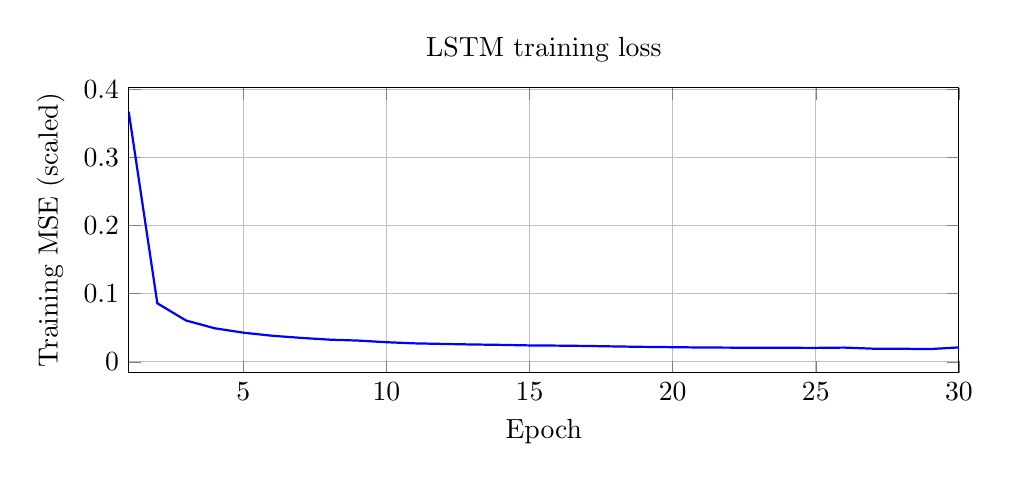
\begin{tikzpicture}\begin{axis}[width=\linewidth,height=5.2cm,xlabel=Epoch,ylabel={Training MSE (scaled)},title={LSTM training loss},xmin=1,xmax=30,grid=major]
\addplot[blue,thick] coordinates {(1,0.367105)(2,0.085854)(3,0.060701)(4,0.049274)(5,0.042806)(6,0.038321)(7,0.035202)(8,0.032585)(9,0.031208)(10,0.028800)(11,0.027091)(12,0.026264)(13,0.025468)(14,0.024889)(15,0.024092)(16,0.023781)(17,0.023304)(18,0.022584)(19,0.021966)(20,0.021509)(21,0.021032)(22,0.020831)(23,0.020699)(24,0.020566)(25,0.020463)(26,0.020898)(27,0.019313)(28,0.019160)(29,0.018752)(30,0.021187)};
\end{axis}\end{tikzpicture}
\end{minipage}\hfill
\begin{minipage}{0.48\linewidth}\centering
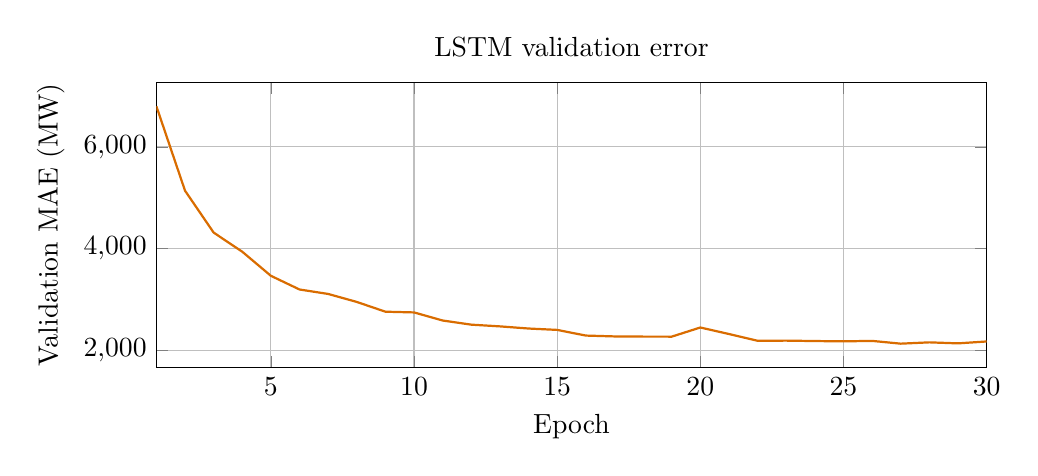
\begin{tikzpicture}\begin{axis}[width=\linewidth,height=5.2cm,xlabel=Epoch,ylabel={Validation MAE (MW)},title={LSTM validation error},xmin=1,xmax=30,grid=major]
\addplot[orange!85!black,thick] coordinates {(1,6798.663)(2,5137.559)(3,4313.185)(4,3936.614)(5,3462.535)(6,3193.648)(7,3105.922)(8,2948.945)(9,2756.675)(10,2742.620)(11,2583.321)(12,2501.938)(13,2468.030)(14,2425.820)(15,2398.766)(16,2287.212)(17,2270.555)(18,2266.797)(19,2266.033)(20,2446.024)(21,2317.703)(22,2184.983)(23,2187.730)(24,2179.538)(25,2173.311)(26,2182.571)(27,2128.005)(28,2153.673)(29,2133.947)(30,2170.927)};
\end{axis}\end{tikzpicture}
\end{minipage}
\caption{User-provided LSTM epoch history. The lowest validation MAE is at epoch 27.}
\end{figure}
\begin{figure}[H]\centering
\IfFileExists{figures/tft\_training\_curve.png}{\includegraphics[width=0.82\linewidth]{figures/tft\_training\_curve.png}}{\fbox{Copy the supplied TFT training curve to figures/tft\_training\_curve.png before compiling.}}
\caption{TFT training curve from the selected trial.}\end{figure}
\section{Phase 4: Results and Evaluation}
\begin{table}[H]\centering\caption{Like-for-like TFT and LSTM results (MW).}\begin{tabular}{llrrl}\toprule Model & Split & MAE & RMSE & Selection/context \\\midrule TFT & Validation & 1,874.62 & 3,616.16 & Larger; validation-MAE selection \\
TFT & Test & 3,542.41 & 6,610.82 & Held-out period \\
LSTM & Validation & 2,128.01 & 3,770.96 & Small; validation-MAE selection \\
LSTM & Test & 4,258.34 & 6,929.33 & Held-out period \\
LSTM & Training & Not recorded & Not recorded & Only scaled training MSE logged \\\bottomrule\end{tabular}\end{table}

TFT has lower reported MAE and RMSE than the supplied LSTM run on both validation and test periods. Test errors exceed validation errors for both models, indicating weaker accuracy on the later holdout. These results describe a single chronological holdout and do not establish that renewable generation caused a change in demand.

The old XGBoost result is excluded from the current research findings and comparison. The attached ZIP's cleaning report lists 12,984 final rows for that run, unlike the 25,678-row TFT/LSTM experiment; its metrics are therefore not presented as comparable evidence.
\section{Contribution Table: Project Modules}
The table below lists the main project modules and their implementation paths. The project team listed on the title page is Abdul Muiz, Abdullah Aftab, and Arqum Umais.
\begin{longtable}{p{0.36\linewidth}p{0.58\linewidth}}\toprule Project module & Implementation files \\\midrule
Data audit and cleaning & \texttt{audit\_india\_dataset.py}; \texttt{clean\_india\_grid.py} \\
TFT model & \texttt{src/models/tft\_model.py} \\
XGBoost implementation (excluded from current findings) & \texttt{src/models/xgboost\_model.py} \\
LSTM model & \texttt{src/models/lstm\_model.py} \\
Report and documentation & \texttt{gridshift\_phase1\_phase4.tex}; \texttt{README.md} \\\bottomrule\end{longtable}
\section{Limitations}
The supplied LSTM run did not report training MAE or RMSE; the available history contains scaled training MSE and validation MAE only. Results reflect one chronological holdout. The earlier XGBoost run used 12,984 rows and is excluded from the 25,678-row TFT/LSTM findings.
\section{References}
\begin{enumerate}[leftmargin=*]
\item Mukherjee, D., Kalita, K., \& Kumar, S. (2025). \textit{Electricity Demand, Solar and Wind Generation Data (September 2021--June 2025) of India at 1-hour interval} (Version 2). Mendeley Data. \url{https://doi.org/10.17632/y58jknpgs8.2}.
\item Hochreiter, S. \& Schmidhuber, J. (1997). Long Short-Term Memory. \textit{Neural Computation, 9}(8), 1735--1780. \url{https://doi.org/10.1162/neco.1997.9.8.1735}.
\item Lim, B., Arik, S. O., Loeff, N., \& Pfister, T. (2021). Temporal Fusion Transformers for Interpretable Multi-horizon Time Series Forecasting. \textit{International Journal of Forecasting, 37}(4), 1748--1764. \url{https://doi.org/10.1016/j.ijforecast.2021.03.012}.
\end{enumerate}
\end{document}
